%%%%%%%%%%%%%%%%%%%%%%%%%%%%%%%%%%%%%%%%%%%%%%%%%%%%%%%%%%%%%%%%%%%%%%%%%%%%%%%%%%%%%%%%%%%%%
%%									Chapitre 4												%
%%%%%%%%%%%%%%%%%%%%%%%%%%%%%%%%%%%%%%%%%%%%%%%%%%%%%%%%%%%%%%%%%%%%%%%%%%%%%%%%%%%%%%%%%%%%%

\chapter{Calcul de Best Matching Unit accéléré avec la topologie}
	\citationChap{
	Il semble que la perfection soit atteinte non quand il n'y a plus rien à ajouter, mais quand il n'y a plus rien à retrancher.
	}{Antoine de Saint-Exupéry}
	\minitoc
	\newpage

%%%%%%%%%%%%%%%%%%%%%%%%%%%%%%%%%%%%%%%%%%%%%%%%%%%%%%%%%%%%%%%%%%%%%%%%%%%%%%%%%%%%%%%%%%%%%



% Début du chapitre			
	\section{Introduction}

	Nous avons dans cette thèse développé des modèles en gardant toujours à l'esprit les contraintes d'une implantation matérielle. Celles-ci impliquent une puissance de calcul limitée et la nécessité d'être réactif en temps réel. Cependant, la quantité de calculs requis par les SOMs est conséquente, que ce soit lors de l'apprentissage ou de la reconstruction. Elle augmente linéairement avec le nombre de neurones, le nombre d'éléments dans le jeu de données et la dimensionnalité de l'entrée. Par conséquent, l'application des SOM à des ensembles de données comportant un grand nombre d'éléments et un nombre élevé de neurones pour représenter précisément l'entrée comme dans notre détection de nouveauté, induit un coût de calcul important qui peut dépasser certaines contraintes telles que le calcul en temps réel ou la faible consommation en énergie. L'optimisation est donc cruciale pour notre approche.

	Des variantes de l'algorithme classique de la SOM ont été développées pour réduire le temps de calcul requis par l'apprentissage. La variante la plus connue est le \textit{batch learning}, comme expliqué dans \cite{cottrell2018self}. Contrairement à l'apprentissage \textit{online} classique, le \textit{batch learning} calcule la moyenne des modifications sur plusieurs vecteurs d'apprentissage avant de mettre à jour les poids des neurones. Des efforts similaires ont été faits dans \cite{fiannaca2013simulated} ou dans \cite{oyana2012new}. Cependant, toutes ces variantes se concentrent uniquement sur la réduction du temps de convergence de l'apprentissage. À notre connaissance, aucun travail n'a été effectué pour réduire le temps nécessaire à chaque itération. Cela peut s'expliquer en partie par la nature hautement parallèle des calculs de distances nécessaires pour chaque itération, si bien que lorsqu'une implantation matérielle rapide est envisagée, la solution est généralement de paralléliser tous ces calculs sur un substrat FPGA avec un circuit dédié pour chaque neurone, comme dans \cite{abadi2018scalable} ou dans \cite{huang2017hardware}. Cependant, l'existence de solutions parallèles ne doit pas conduire à un manque d'effort dans l'optimisation des algorithmes, car la majorité des applications de la SOM sont sur CPU, sans parallélisation, et que les implantations des SOM dans les systèmes embarqués sont souvent limitées par la place disponible sur le FPGA, la consommation électrique ou la vitesse de traitement, qui peuvent tous être améliorés par l'utilisation d'algorithmes d'apprentissage plus efficaces.

	Une itération comprend deux phases, la recherche de la BMU et la modification des poids. Nous nous intéresserons ici à la recherche de BMU uniquement, car utile aussi après l'apprentissage. Traditionnellement, la BMU est déterminée par une recherche exhaustive en comparant toutes les distances entre le vecteur d'entrée et les prototypes des neurones. Cette méthode, bien qu'elle permette de toujours trouver le bon minimum dans la carte, est inefficace en calculs, car contrairement aux k-means par exemple, les neurones d'une SOM ne sont pas indépendants entre eux, et l'information présente dans la topologie de la SOM peut être exploitée. 
	
	Comme pour la détection de nouveauté, nous avons de nouveau utilisé la propriété de réduction dimensionnelle des SOM pour cette fois-ci accélérer la recherche de la BMU. Pour rappel, la réduction dimensionnelle signifie que les neurones proches dans la topologie de la SOM représentent des vecteurs proches dans l'espace d'entrée. Par conséquent, lorsque l'on calcule les distances de tous les neurones avec un vecteur d'entrée, un gradient pseudo-continu apparaît dans la SOM dont le minimum est situé à la best matching unit. En utilisant une approche à base de descente de gradient discrétisée, on peut alors s'attendre à pouvoir atteindre la BMU de la carte, en ne devant calculer qu'une partie seulement des distances entre le vecteur d'entrée et les vecteurs prototypes des neurones. Ce principe est la base de notre algorithme de recherche de BMU que nous appellerons ici FastBMU. Avec notre méthode, nous explorons une nouvelle approche pour l'optimisation des SOM qui peut être combinée avec d'autres méthodes d'optimisation couramment utilisées dans ces modèles pour un calcul encore plus rapide dans les phases d'apprentissage et de rappel.

	Ce chapitre est découpé en deux sections. La première présente l'algorithme et son fonctionnement détaillé dans le cas séquentiel. Cette section inclut également une analyse de la complexité et une évaluation des performances et des gains en calculs obtenus. La seconde partie présente l'adaptation de cet algorithme dans le cas parallèle, pour les implantations matérielles.

	\newpage

	\section{Algorithme séquentiel}\label{sec:fast:seq}

	Pour bien comprendre le fonctionnement de notre algorithme Fast-BMU, nous allons le présenter partie par partie. Nous commencerons par l'idée générale de la descente du gradient de la SOM. Puis nous aborderons les cas spéciaux en expliquant pourquoi ils existent, les conséquences possibles et comment Fast-BMU les résout.

	\begin{algorithm}
	\caption{Particule}
	\label{fast:alg:particle}
	\DontPrintSemicolon
	\Entree{\;
	{\tt vecteur} : vecteur d'entrée \;
	{\tt pos}: position de la particule}
	\Donnees{\;
	{\tt memoire\_dist}: historique des distances déjà évaluées\;}
	\Sortie{\;
	{\tt bmu} : index de la Best Matching Unit potentielle\;\;}

	\Deb{
		\tcp{On commence par regarder les voisins directs pour trouver si l'un}
		\tcp{d'entre eux est plus proche du vecteur d'entrée.}
		{\tt bmu\_voisin} $\leftarrow$ RechercheVoisin({\tt vecteur}, {\tt pos}, 1)\;
		\Si{{\tt memoire\_dist[bmu\_voisin]} $<$ {\tt memoire\_dist[\tt pos]}}{
			\Retour{Particule({\tt vecteur}, {\tt bmu\_voisin})}
		}
		\tcp{Si il n'y en a pas, alors on se trouve dans un minimum local.}
		\tcp{On effectue alors une nouvelle recherche dans le voisinage de 2.}
		{\tt bmu\_voisin} $\leftarrow$ RechercheVoisin({\tt vecteur}, {\tt pos}, 2)\;
		\Si{{\tt memoire\_dist[bmu\_voisin]} $<$ {\tt memoire\_dist[\tt pos]}}{
			\Retour{Particule({\tt vecteur}, {\tt bmu\_voisin})}
		}
		\tcp{Si on ne trouve toujours rien, alors on peut considérer que l'on a atteint}
		\tcp{la fin de la descente de gradient.}
		\Retour{{\tt pos}}
	}
	\end{algorithm}

	\begin{algorithm}
	\caption{RechercheVoisin}
	\label{fast:alg:voisin}
	\DontPrintSemicolon
	\Entree{\;
	{\tt vecteur} : vecteur d'entrée \;
	{\tt pos}: position de la particule\;
	{\tt x}: distance topologique}
	\Donnees{\;
	{\tt resultats}: dictionnaire vide\;
	{\tt prototypes}: valeurs des vecteurs prototypes de la SOM\;
	{\tt memoire\_dist}: historique des distances déjà évaluées\;}
	\Sortie{\;
	{\tt bmu} : index de la Best Matching Unit potentielle\;\;}

	\Deb{
		\Pour{{\tt voisin} dans le voisinage à distance topologique x de {\tt pos}}{
			\Si{{\tt memoire\_dist[voisin]} est vide}{
				{\tt memoire\_dist[voisin]} $\leftarrow$ distance({\tt prototypes[voisin]}, {\tt vecteur})\;
				{\tt resultats[\tt voisin]} $\leftarrow$ {\tt memoire\_dist[voisin]}\;
			}
		}
		{\tt bmu\_voisin} $\leftarrow$ minimum de {\tt resultats}\;
		\Retour{{\tt bmu\_voisin}}
	}
	\end{algorithm}

	Le cœur de Fast-BMU est la descente de gradient discrétisée sur les neurones qui minimise la distance entre ceux-ci et le vecteur d'entrée. Le pseudo-code de cette descente de gradient, appelée \textit{Particule}, est présenté dans les algorithmes \ref{fast:alg:particle} et \ref{fast:alg:voisin}. Une \textit{Particule} commence à une position choisie arbitrairement dans la carte. Pour cet exemple, illustré dans la figure \ref{fig:first_particle}, considérons qu'elle débute aux coordonnées (0,0) (coin supérieur gauche). Ce neurone a deux voisins, un à l'est (1,0) et un au sud (0,1). Nous évaluons les distances au vecteur d'entrée de ces trois neurones pour trouver la prochaine étape de la descente du gradient. Si l'un des neurones voisins donne la plus petite distance, alors la descente du gradient va dans la direction de ce neurone particulier, qui devient la prochaine position sélectionnée à partir de laquelle nous répétons ce processus. Si la plus petite distance est trouvée là où nous sommes actuellement positionnés, alors nous considérons que nous nous trouvons dans un minimum local. Dans notre exemple, la plus petite distance est mesurée pour le neurone situé à l'est en (1,0). Le processus de recherche se déplace donc d'un pas vers l'est. Ce neurone a trois voisins, un au sud (1,1), un à l'est (2,0) et un à l'ouest dont nous venons et que nous allons donc ignorer. Nous comparons à nouveau les trois distances et nous nous déplaçons vers la distance la plus faible (le Sud). Ce processus itère jusqu'à atteindre un minimum local à la position (6,5), où tous les neurones voisins ont une distance au vecteur d'entrée plus élevée que le neurone sélectionné.

	Trouver un neurone sans meilleurs voisins ne garantit cependant pas que l'on a terminé la descente de gradient. On peut observer par exemple sur la figure \ref{fig:first_particle} que les neurones au sud et à l'ouest du premier minimum local ont un gradient qui pointent vers un autre neurone que le minimum local actuel. Cela s'explique par le fait que, surtout pour les topologies en grille, le gradient soit localement orienté en diagonale, et que par conséquent il faille deux étapes (sud puis ouest ou ouest puis sud) pour continuer la descente. Pour compenser ce problème, et afin de s'assurer que le minimum local qui a été trouvé est bien le meilleur dans le voisinage local, nous effectuons une recherche de minimum dans tous les voisins à voisinage topologique de 2. Si un nouveau minimum a été trouvé, nous continuons la descente de gradient à partir de celui-ci. Si il n'y en a pas, alors nous considérons que la descente de gradient est terminée, et que la position actuelle est le minimum trouvé. Car tous ses voisins sont moins bons, et que le gradient de tous ses voisins amènent à lui.

	\begin{figure}[!t]
    	\centering
    	\includesvg[scale=1.2]{first_particle}\ \ \ \ \ \ \ 
    	\includesvg[scale=1.2]{all_particles}
		\caption[Visualisation de l'algorithme de particule]{À Gauche : exemple d'exécution d'une particule. Chaque cellule représente un neurone. La flèche dans chaque cellule pointe vers le meilleur voisin (qui a une distance inférieure). Une étoile représente un minimum local. Les cellules vertes sont les neurones qui ont été explorés pendant la recherche, et les cellules bleues sont les neurones dont la distance au vecteur d'entrée a été calculée mais qui n'ont pas été sélectionnés par l'algorithme. Après avoir trouvé un minimum local, de nouvelles particules sont créées (en rouge) et continuent la descente du gradient en explorant le voisinage local. La cellule en jaune est la BMU, et le minimum global de la carte. À droite : exécution des quatre particules.}
    	\label{fig:first_particle}
	\end{figure}

	Un autre problème qui peut survenir avec une unique \textit{Particule} est dû aux bords. Lors de la projection de données à haute dimension sur une SOM 2D, la carte peut parfois devenir tordue sans gradient continu entre le neurone supérieur gauche et le neurone inférieur droit. Imaginez par exemple un filet que l'on jette sur une sphère et qui l'enveloppe presque complètement : le chemin le plus court entre un coin du filet et le coin opposé du filet ne suivra pas les mailles du filet. Si, au cours de la phase d'apprentissage, la particule se retrouve dans le mauvais coin de la SOM, elle trouvera une très mauvaise BMU et la mise à jour des vecteurs prototypes des neurones brisera localement la continuité du voisinage, et créera une boucle de rétroaction négative qui détruira toutes les propriétés de réduction dimensionnelles de la SOM. Il existe un moyen facile d'éviter cela, en démarrant 4 \textit{Particules}, une dans chaque coin de la SOM, et en sélectionnant la plus petite BMU trouvée parmi les 4. Cette technique préserve la continuité du SOM et rend l'algorithme Fast-BMU plus robuste aux discontinuités locales du gradient, notamment au début de l'apprentissage, lorsque la carte n'est pas encore bien déployée. Fast-BMU complet est défini dans l'algorithme \ref{fast:alg:bmu}, et le résultat d'une exécution complète est illustré dans la figure \ref{fig:first_particle} à droite.
	
	Il faut aussi remarquer que dans le cas où il n'y a pas de gradient clair dans la SOM (typiquement lorsque la SOM est initialisée de façon aléatoire avant l'apprentissage), Fast-BMU ne trouvera pas la BMU correcte. Toutefois, ce n'est pas un problème pour l'apprentissage, car la fonction de voisinage créera un gradient en dépliant la SOM, quel que soit le neurone initialement sélectionné, et une fois le gradient créé, Fast-BMU trouvera les bonnes BMU.

	\begin{algorithm}
	\caption{FastBMU}
	\label{fast:alg:bmu}
	\DontPrintSemicolon
	\Entree{\;
	{\tt vecteur} : vecteur d'entrée \;
	{\tt l, h}: largeur et hauteur de la SOM}
	\Donnees{\;
	{\tt positions}: positions de départ des particules\;
	{\tt memoire\_dist}: historique des distances déjà évaluées\;
	{\tt resultats}: dictionnaire vide}
	\Sortie{\;
	{\tt bmu} : index de la Best Matching Unit\;\;}

	\Deb{
		{\tt positions} $\leftarrow [(0,0), (l-1, 0), (0, h-1), (l-1, h-1)]$\;
		\Pour{{\tt pos} dans {\tt positions}}{
			{\tt bmu\_particule} = Particule({\tt vector}, {\tt pos})\;
			{\tt resultats[bmu\_particule]} $\leftarrow$ {\tt memoire\_dist[bmu\_particule]}\;
		}
		{\tt bmu} = minimum de {\tt resultats}\;
		\Retour{{\tt bmu}}
	}
	\end{algorithm}

	\subsection{Analyse de la complexité}\label{seq:complex_analysis}

	Le temps d'exécution d'une recherche de BMU dans la SOM classique dépend de deux facteurs : le nombre de neurones multiplié par la durée d'une comparaison entre le vecteur d'entrée et les poids d'un neurone. L'idée de Fast-BMU étant de réduire le nombre de ces comparaisons, la durée d'une comparaison ne sera pas prise en compte dans cette analyse. C'est normalement une valeur qui ne dépend que de la dimensionnalité des données. Le nombre de comparaisons pour Fast-BMU est quant à lui dépendant de la taille de la carte, c'est à dire hauteur et largeur, et de la topologie, c'est à dire du nombre de voisins par neurone. 

	Nous ferons dans cette analyse l'hypothèse qu'il y a une certaine continuité dans la carte et qu'en partant de n'importe quel point de la carte, on atteigne la BMU en suivant le gradient sans revenir en arrière, c'est à dire que la distance parcourue en suivant le gradient entre les deux soit égale à la distance de manhattan. C'est une hypothèse forte, mais qui doit être vraie pour que notre algorithme de Fast-BMU fonctionne. En pratique, Fast-BMU est plus robuste que cela, et n'a pas besoin que tous les gradients de la carte mènent à la BMU, il en faut juste assez pour qu'une \textit{particule} la trouve. De plus, les problèmes les plus communs dans le gradient de la carte sont des minimums locaux, qui réduisent le nombre de \textit{pas} en arrêtant la \textit{particule} avant la fin. Pour augmenter le nombre de pas effectués par une particule, il faudrait un gradient qui prenne une direction à l'opposé de ce qu'il avait précédemment. Qu'il fasse des méandres sur son trajet par exemple, ce qui est inhabituel dans des SOM en général. Ainsi, la complexité que nous allons calculer sera probablement une limite haute à la vraie complexité de l'algorithme Fast-BMU. 

	Pour estimer la complexité de notre algorithme, c'est à dire le nombre de comparaisons dans notre cas, nous devons estimer le nombre de \textit{pas} de chaque particule pour trouver la BMU potentielle. En considérant que la BMU est localisée à la position $x, y$ de la SOM, on a :
	\begin{itemize}
    	\item La \textit{particule} en haut à gauche commençant aux coordonnées $0, 0$ devra faire $x$ \textit{pas} horizontaux et $y$ \textit{pas} verticaux pour atteindre la BMU.
		\item De la même façon, la \textit{particule} du haut à droite avec les coordonnées $(w,0)$ devra faire $w-x$ \textit{pas} horizontaux et $y$ pas verticaux.
		\item Pour la \textit{particule} en bas à gauche $(0,h)$, ce sera $x$ et $h-y$ \textit{pas}.
		\item Pour la \textit{particule} en bas à droite $(w,h)$, ce sera $w-x$ et $h-y$ \textit{pas}.
	\end{itemize}

	Pour obtenir le nombre total de \textit{pas} pour une itération, nous additionnons les nombres de pas de toutes les particules ensemble comme montré dans l'équation \ref{fast:eq:nbsteps}.

	\begin{equation}\label{fast:eq:nbsteps}
	\begin{split}
    	\text{NbrPas} &= (x + y) + (w - x + y) + (x + h - y) + (w - x + h - y)\\
		&= 2x - 2x + 2y - 2y + 2w + 2h 
	\end{split}
	\end{equation}

	Les $x$ et $y$ s'annulant, le nombre total de pas ne dépend donc que de la largeur et la hauteur de la carte, soit $(2w + 2h)$. On peut donc en déduire la Complexité Estimée $\cal C$ avec l'équation \ref{fast:eq:complexity}

	\begin{align}\label{fast:eq:complexity}
    	{\cal C}(w, h) = 2 \times (w + h) \times \textit{NbrEvalParPas}
	\end{align}

	avec $w, h$ la largeur et la hauteur de la SOM respectivement et \textit{NbrEvalParPas} le nombre de nouvelles distances à calculer pour chaque \textit{pas} d'une particule. Sa valeur dépend de la topologie. Elle est au maximum de 3 avec une grille (4 voisins moins le neurone de l'étape précédente) et également de 3 avec une topologie hexagonale (6 voisins moins le neurone de l'étape précédente et 2 neurones qui étaient voisins du neurone précédent et qui ont donc déjà été évalués). 

	D'un point de vue analytique, nous pouvons estimer que notre algorithme Fast-BMU (${\cal C}(w,h)=6(w+h)$ dans le pire des cas dans une configuration de grille standard) est significativement plus rapide que l'algorithme actuel de recherche exhaustive (O$(w,h) = wh$) lorsque le nombre de neurones dans la carte est important. Par exemple, il est théoriquement deux fois plus rapide avec des SOM de 24 par 24, et 10 fois plus rapide avec des SOM de 120 par 120. Une évaluation expérimentale de la différence de vitesse est présentée dans la section \ref{fast:seq:gain_comput}.

	\subsection{Protocole expérimental}\label{seq:exp}

	En pratique, il arrive parfois malgré tout que FastBMU se trompe de BMU. Nous allons donc expérimentalement mesurer l'impact de ces erreurs sur l'apprentissage et la reconstruction. Pour évaluer la robustesse de notre algorithme avec différents types de données, nous avons sélectionné 6 jeux de données représentatifs du type de données sur lesquelles les SOM sont habituellement entraînés. Pour le cas 2D, nous avons généré des données avec différentes propriétés (une distribution uniforme et une forme hautement non convexe), pour les données 3D nous utilisons une forme cubique uniformément distribuée et les valeurs de couleur des pixels d'une image. Pour les hautes dimensions, nous considérons l'apprentissage par imagettes d'une image tel qu'il a déjà été présenté, avec des sous-images de 10 par 10 comme vecteurs d'entraînement (100 pixels avec 3 couleurs chacun, ce qui donne 300 dimensions), ainsi que le Free Spoken Digits Dataset \cite{zohar_jackson_2018_1342401} qui utilise des ondes sonores que nous avons réduites à 1000 dimensions. Nous emploierons des SOM à 2 dimensions avec des topologies en grille et hexagonales, car ce sont les plus utilisées.

	Pour ces tests, nous avons fait débuter $\alpha$ à 0.6 pour finir à 0.05. $\sigma$ commence à 0.5 et termine à 0.001. La SOM est de taille $32\times32$ (1024 neurones) et apprend pendant 10 époques.

	Afin d'évaluer les différences entre tous les modèles testés, nous avons utilisé deux métriques. La première est la \textit{Mean Squared Quantization Error} (MSQE) que nous avons déjà utilisée dans le chapitre 2. MSQE mesure la qualité de quantification vectorielle de l'algorithme testé. La seconde métrique est la \textit{Mean Squared Distance to Neurons} (MSDtN) qui calcule la distance moyenne au carré entre les prototypes des neurones et ceux de leurs voisins directs. Plus cette valeur est faible, plus les neurones voisins sont proches dans l'espace d'entrée et plus la propriété de réduction dimensionnelle est bonne. De nombreuses métriques existent dans la littérature sur les SOM pour la qualité de la réduction dimensionnelle d'une SOM \cite{polzlbauer2004survey}, mais MSDtN a l'avantage d'être facile à calculer, sans paramètres et de ne dépendre que des poids des neurones. Pour les deux métriques retenues, une valeur plus faible est meilleure. 

	\begin{equation}
		\text{MSQE} = \frac{1}{dn} \sum_{i=0}^{n-1} (v_i - w_\textit{bmu(i)})^2
	\end{equation}

	\begin{equation}
    	\text{MSDtN} = \frac{1}{dN} \sum_{i=1}^{N} \sum_{j=1}^{N} 
    	\begin{cases}
        	(w_i - w_j)^2,  & \text{Si dist}(i, j) = 1\\
        	0,              & \text{Sinon}
    	\end{cases}
	\end{equation}

	Avec $n$ étant le nombre de vecteurs dans le jeu de données, $d$ leur dimensionnalité, $v_i$ le $i^{ème}$ vecteur d'entrée, et bmu($i$) l'indice du neurone qui est la \textit{best matching unit} de $v_i$. De même, $N$ est le nombre de neurones de la SOM et $w_i$ les poids du $i^{ème}$ neurone, tandis que dist($i, j$) est le nombre de connexions dans le chemin le plus court entre les neurones $i$ et $j$ dans la carte neuronale.

	\subsection{Résultats}
	\subsubsection{Performances}

	Dans cette section, nous examinerons les différences de qualité d'apprentissage et de reconstruction entre la version standard et notre version FastBMU pour le calcul de la BMU. Nous regarderons également les différences pratiques dans le nombre de calculs requis pour les deux versions et nous les comparerons avec l'analyse de complexité présentée précédemment.

	Pour chaque combinaison de jeu de données et de modèle (choix de la topologie et de l'algorithme BMU), nous avons effectué 50 exécutions avec différentes graines aléatoires qui affectent les jeux de données générés, l'initialisation des poids des neurones (qui sont tous initialisés aléatoirement sans gradient préexistant) et l'ordre dans lequel les vecteurs d'apprentissage sont présentés. Les résultats sont présentés dans le tableau \ref{tab:fast:res}.

	La colonne apprentissage du tableau indique la combinaison de l'algorithme de recherche de BMU et de la topologie qui a été utilisée pour l'entraînement. La MSDtN (voir section \ref{seq:exp}) est calculée sur les poids des neurones entraînés. La MSQE\_S (Standard) est l'erreur de quantification dans la phase de reconstruction (après apprentissage) en utilisant la recherche de BMU standard. La comparaison des différentes valeurs de MSQE\_S pour des SOM ayant été apprises par une version standard et une version rapide de la recherche de BMU donne une indication de l'influence de l'algorithme Fast-BMU sur la qualité de l'apprentissage uniquement, car il sélectionne toujours la vraie BMU dans la phase de reconstruction. La métrique MSQE\_F (Fast) mesure l'erreur de quantification vectorielle avec la sélection de BMU effectuée par l'algorithme Fast-BMU. Si l'entraînement a été effectué sur la SOM standard, il donne une indication de l'influence de l'algorithme Fast-BMU sur la précision du reconstruction uniquement ; s'il a été entraîné sur une version Fast, il représente le résultat MSQE d'une SOM qui utilise uniquement l'algorithme Fast-BMU. La colonne \textit{Mismatch} donne la proportion de BMU qui sont sélectionnées différemment par les deux algorithmes.

	\begin{tableth}
	\caption[Résultats de FastBMU sur différentes données]{Résultats avec une SOM de $32\times32$ neurones, avec 50 executions par ligne. La colonne \textit{Apprentissage} précise avec quel algorithme et quelle topologie la SOM a été entraînée. MSQE\_S est le MSQE calculé après apprentissage avec l'algorithme BMU standard (exhaustif) tandis que MSQE\_F utilise la version Fast-BMU. Nous combinons les deux apprentissages avec les deux reconstructions possibles (Standard et Fast). Les différences de MSQE\_S entre les différents algorithmes reflètent ainsi la qualité de la phase d'apprentissage. Le \textit{Mismatch} est la proportion de BMU qui sont sélectionnés différemment par les deux algorithmes.}
	\begin{tabular}{|c|l|r|r|r|r|}
	\hline
	Données & Apprentissage & MSDtN & MSQE\_S & MSQE\_F & Mismatch\\
	\hline
	Carré 	& Grille  & \nbr{1.94e-4} & \nbr{2.22e-4} & \nbr{2.22e-4} & 0\%\\
    (2D)   	& Fast-Grille & \bst{1.93e-4} & \nbr{2.23e-4} & \nbr{2.23e-4} & 0\%\\
        	& Hexagonal	& \nbr{2.39e-4} & \bst{2.12e-4} & \bst{2.12e-4} & 0\%\\
        	& Fast-Hexa	& \nbr{2.38e-4} & \nbr{2.15e-4} & \nbr{2.15e-4} & 0\%\\
	\hline
	Forme   & Grille  & \bst{1.38e-4} & \nbr{1.40e-4} & \nbr{1.40e-4} & $\approx$0\%\\
    (2D)    & Fast-Grille & \bst{1.38e-4} & \nbr{1.40e-4} & \nbr{1.40e-4} & $\approx$0\%\\
        	& Hexagonal   & \nbr{1.65e-4} & \bst{1.31e-4} & \bst{1.31e-4} & $\approx$0\%\\
        	& Fast-Hex & \nbr{1.65e-4} & \bst{1.31e-4} & \bst{1.31e-4} & $\approx$0\%\\
	\hline
	Cube   	& Grille  & \bst{4.48e-4} & \nbr{2.21e-3} & \nbr{2.50e-3} & 4.8\%\\
    (3D)   	& Fast-Grille & \nbr{4.61e-4} & \nbr{2.25e-3} & \nbr{3.21e-3} & 9.8\%\\
        	& Hexagonal   & \nbr{5.29e-4} & \bst{2.09e-3} & \bst{2.34e-3} & \bf{3.1\%}\\
        	& Fast-Hex & \nbr{5.38e-4} & \nbr{2.11e-3} & \nbr{2.79e-3} & 7.6\%\\
	\hline
	Couleurs& Grille  & \bst{1.15e-4} & \nbr{8.64e-5} & \nbr{8.80e-5} & 4.4\%\\
    (3D)    & Fast-Grille & \nbr{1.19e-4} & \nbr{8.91e-5} & \nbr{9.08e-5} & 5.4\%\\
        	& Hexagonal   & \nbr{1.33e-4} & \nbr{8.29e-5} & \nbr{8.30e-5} & \bf{0.4\%}\\
       		& Fast-Hex & \nbr{1.35e-4} & \bst{8.26e-5} & \bst{8.29e-5} & 0.7\%\\
	\hline
	Image  	& Grille  & \bst{1.64e-4} & \nbr{1.80e-3} & \nbr{1.83e-3} & 4.2\%\\
    (300D)    & Fast-Grille & \nbr{1.65e-4} & \nbr{1.82e-3} & \nbr{1.85e-3} & 4.4\%\\
        	& Hexagonal   & \nbr{1.97e-4} & \bst{1.75e-3} & \nbr{1.77e-3} & \bf{1.2\%}\\
        	& Fast-Hex & \nbr{1.99e-4} & \bst{1.75e-3} & \bst{1.76e-3} & \bf{1.2\%}\\
	\hline
	Sons    & Grille  & \nbr{2.02e-4} & \nbr{1.42e-2} & \nbr{1.49e-2} & 31.3\%\\
    (1000D)   	& Fast-Grille & \bst{1.93e-4} & \nbr{1.44e-2} & \nbr{1.51e-2} & 32.2\%\\
        	& Hexagonal   & \nbr{2.29e-4} & \bst{1.41e-2} & \bst{1.45e-2} & 19.8\%\\
        	& Fast-Hex & \nbr{2.25e-4} & \nbr{1.42e-2} & \bst{1.45e-2} & \bf{13.3\%}\\
	\hline
	\end{tabular}
	\label{tab:fast:res}
	\end{tableth}

	Nous observons d'abord que la distance entre les neurones après apprentissage (MSDtN) est plus faible avec la topologie en grille qu'avec la topologie hexagonale, mais cette différence pourrait être attribuée au nombre différent de voisins entre les deux topologies et ne devrait donc être utilisée que pour comparer les différences entre les algorithmes standard et Fast-BMU, et pas les topologies. Nous remarquons également que l'algorithme Fast ne présente pas d'écart significatif sur les jeux de données Square et Shape, et donc que MSQE\_S et MSQE\_F ont des résultats de reconstruction similaires sur ces jeux de données.

	Les pourcentages de \textit{mismatch} varient considérablement d'un ensemble de données à l'autre. De 0 à 6\% pour les jeux de données Images et Couleurs, de 3 à 10\% pour le Cube et de 13 à 33\% pour les données sonores. Ces différences peuvent s'expliquer par la distribution des données d'entrée, car les jeux de données Images et Couleurs contiennent des éléments qui sont étroitement liés entre eux. Dans les images, par exemple, il y a généralement quelques couleurs dominantes avec beaucoup de valeurs intermédiaires qui rendent les continuités de la distribution plus faciles à réduire dimensionnellement pour une SOM, améliorant ainsi les performances de notre algorithme Fast-BMU. En revanche, le jeu de données \textit{Spoken Digits} présente des valeurs de \textit{mismatch} élevées, ce qui semble indiquer qu'une forte continuité dans les poids des neurones n'est pas présente après l'apprentissage. La topologie hexagonale est également plus performante avec l'algorithme Fast-BMU que la topologie en grille, car les \textit{mismatch} sont nettement plus faibles avec elle. Enfin, la dimensionnalité d'un jeu de données ne semble pas jouer un rôle clé ici, puisque le jeu de données Image (300 dimensions) présente moins de \textit{mismatch} que le jeu de données Cube (3 dimensions).

	Pour la partie quantification vectorielle, la topologie hexagonale donne à nouveau les valeurs d'erreur les plus faibles. Ce qui est plus surprenant, c'est que la version Fast-BMU présente des résultats de quantification très similaires à ceux de la version standard. Même avec des \textit{mismatch} élevés (30\% avec Digits utilisant un SOM basé sur une grille), le MSQE n'est supérieur que d'environ 5\%, et encore moins lorsque seul l'apprentissage est comparé. Les seules valeurs de MSQE significativement plus élevées avec Fast-BMU concernent le jeu de données Cube, où l'algorithme sélectionne de très mauvais choix de BMU dans la phase de reconstruction tout en étant capable de former correctement la SOM. Dans la plupart des cas, une différence dans la topologie de la SOM a plus d'impact sur la MSQE que l'utilisation de l'algorithme Fast-BMU.

	\subsubsection{Gains computationnels}\label{fast:seq:gain_comput}

	\begin{figureth}
    	\centering
    	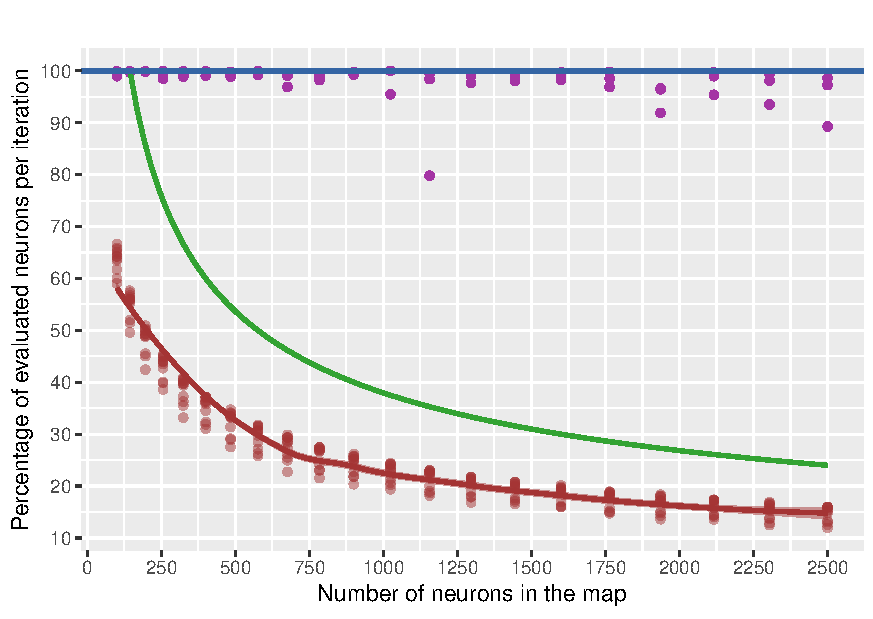
\includegraphics[width=1\textwidth]{performance_diff.pdf}
	%    \includesvg[inkscapelatex=false, width=0.8\textwidth]{performance_diff.pdf}
    	\caption[Évaluation des gains de performance en fonction du nombre de neurones]{Évaluation des gains de quantité de calculs en fonction du nombre de neurones. Le gain en performance est exprimé en pourcentage de neurones qui ont dû être évalués pendant la recherche de BMU. Tous les résultats ont été calculés sur des cartes carrées. La ligne bleue représente la SOM standard, en vert la valeur analytique calculée et en rouge la valeur mesurée. En outre, les points violets représentent le pourcentage de BMU correctes dans une exécution sur le jeu de données Image.}
    	\label{fig:performance_diff}
	\end{figureth}

	Pour évaluer les gains de calcul induits par l'utilisation de l'algorithme Fast-BMU indépendamment des techniques d'implémentation, nous avons comparé le pourcentage de neurones qui doivent être évalués afin de trouver le BMU. Les résultats sont présentés dans la figure \ref{fig:performance_diff}. La SOM standard évalue par définition tous les neurones, le pourcentage est donc toujours de 100\%. La courbe de complexité de Fast-BMU représente la fonction définie dans la section \ref{seq:complex_analysis}. Pour obtenir la courbe mesurée par Fast, nous avons effectué des tests avec des SOM de taille $n\times n$, où $n$ est tout nombre pair compris entre 10 et 50 (21 tests au total). Chaque test comprenait tous les ensembles de données et toutes les topologies (soit 12 exécutions par test).

	Notre algorithme est deux fois plus rapide avec des SOM de $16\times16$, quatre fois plus rapide avec 1000 neurones ($32\times32$). La SOM $50\times50$ évalue environ 375 neurones par itération, ce qui est similaire aux 400 neurones qu'une SOM standard de $20\times20$ doit évaluer. Nous pouvons également observer que la courbe de complexité suit une forme similaire à la courbe mesurée, tout en surestimant le nombre requis de neurones évalués d'environ 75\%.

	\newpage
	\section{Algorithme parallèle}

	Une implémentation matérielle sur FPGA de notre détection de nouveauté nécessiterait du parallélisme pour utiliser efficacement les ressources à disposition. Car implémenter une SOM complète sur FPGA pour n'avoir qu'une dizaine de neurones actifs en même temps serait sous optimal. FastBMU est cependant un algorithme fondamentalement séquentiel. Chaque étape de celui-ci dépend fortement de l'étape précédente pour suivre le gradient. Par conséquent en faire une version parallèle nécessiterait de changer fondamentalement son fonctionnement. Une idée plus simple pour réaliser ce parallélisme serait de le placer non pas au niveau de la recherche de BMU, mais au niveau des itérations. En effet, si il est possible de paralléliser les instructions d'une façon qui permette d'utiliser quasiment tous les neurones simultanément avec FastBMU sans compromettre la qualité des BMU trouvées, alors nous aurons un moyen d'être plus performant que les versions purement parallèles de SOM qui calculent les distances de tous les neurones en une seul étape. Si nous atteignons un pourcentage d'utilisation par neurone proche de 100\%, en utilisant FastBMU qui fait beaucoup moins d'évaluations que la version standard, alors nous calculerons plus de BMU par étape que la version standard parallèle.

	\subsection{Adaptation pour le parallélisme}

	Une des propriétés de FastBMU, est qu'il part des quatre coins et qu'il converge vers le centre pendant son exécution. Ce qui veut dire que l'utilisation des neurones se fait par vague. Ainsi on si on lance une itération de FastBMU par étape, on utilisera de façon plus efficiente les neurones. Lancer une itération par étape donnera une vitesse équivalente pour FastBMU en parallèle à la version standard en parallèle. Mais avec FastBMU, les poids des neurones pourront changer pendant la descente de gradient, puisque ce sont les itérations qui sont dorénavant parallélisées.

	L'intérêt de FastBMU étant de réduire le nombre d'évaluations effectuées par recherche de BMU, envoyer une itération par étape ne suffira pas à saturer les neurones, et il existera toujours des neurones inactifs grâce aux évaluations évitées. Mais on ne peut pas simplement envoyer plus d'itérations par étape, car nous savons que les neurones dans les coins par exemple sont utilisés à 100\%, car ce sont les points de départ des particules. Nous avons donc calculé le pourcentage d'utilisation de tous les neurones dans la figure \ref{fig:fast:eval_percent}. Les valeurs de la figure proviennent d'un exemple particulier d'une carte de 20 par 20 neurones, mais les catégories sont généralisables pour tout types de données et pour toutes les tailles de carte assez grandes, tant qu'un gradient est présent pour que FastBMU fonctionne.

	\begin{figureth}
    	\centering
    	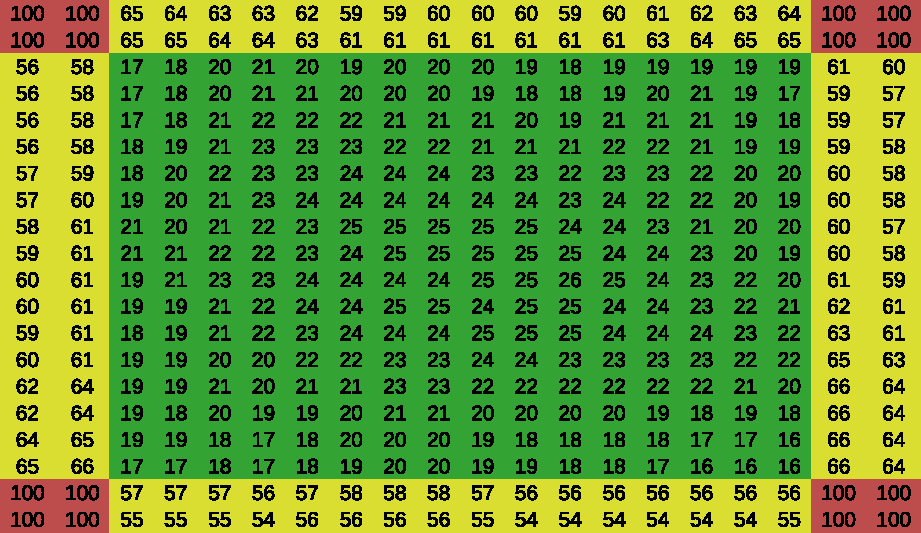
\includegraphics[width=.9\textwidth]{utilisation.pdf}
    	\caption[Pourcentage d'évaluations par neurones pour FastBMU]{Pourcentage d'évaluations par neurones pour FastBMU. On peut diviser ceux-ci en trois catégories. La première en rouge regroupe tous les coins qui sont évalués à chaque itération, puisque point de départ des particules. La seconde sont les bords en jaune qui sont évalués un peu plus de la moitié du temps. La dernière est le centre en vert, qui sont évalués moins d'un quart du temps.}
    	\label{fig:fast:eval_percent}
	\end{figureth}

	D'après la figure, on peut diviser les neurones en trois catégories, les coins, les bords et le centre. Les coins étant utilisés 100\% du temps, les bords entre 50 et 60\% du temps et moins de 25\% du temps pour les neurones centraux. Ainsi, pour augmenter l'utilisation des neurones proche des 100\%, il faut multiplier l'utilisation des neurones centraux par 4. Pour ce faire il est nécessaire d'augmenter le nombre d'itérations commencées par étape à 4. Cependant cela augmentera l'utilisation des neurones des bords et des coins au delà de 100\%. Pour résoudre ce problème, il est possible d'augmenter matériellement le nombre de comparaisons que peuvent effectuer ces neurones. Si l'on multiplie par 4 le nombre de comparaisons simultanées que l'on peut faire pour les neurones de chaque coin par exemple, ils pourront traiter 4 itérations simultanément, et seront capables de gérer la surcharge nécessaire pour augmenter l'efficacité des neurones centraux. Le même principe peut être appliqué pour les neurones des bords, en leur permettant de faire deux ou trois comparaisons simultanées.

	Ces valeurs pourraient changer avec la taille de la carte. Une carte plus grande utilisera moins d'évaluations par recherche de BMU, et les pourcentages d'utilisation des neurones centraux diminueront en conséquence. Les neurones des bords et des coins resterons eux à des pourcentages similaires. Des cartes plus grandes nécessiteront donc de faire plus d'itérations par étape si l'on souhaite garder des neurones centraux proche des 100\% d'utilisation. Le nombre d'évaluations parallèles possibles par les neurones des bords et des coins devront aussi être augmentés.

	En lançant 4 nouvelles itérations par étape, nous devenons plus performants que la version classique de la SOM parallèle, qui ne peut faire qu'une itération par étape. Mais il reste la question de l'impact qu'a la modification des poids des neurones pendant que des descentes de gradient sont en cours. Nous l'évaluerons dans la section suivante.

	\subsection{Evaluation}

	Nous avons évalué les performances de notre algorithme parallèle de la même manière que la version séquentielle, avec quelques données en moins. Les résultats sont présentés dans le tableau \ref{tab:fast:parallel}. Ils ne sont cependant pas directement comparables avec ceux montrés précédemment dans le tableau \ref{tab:fast:res}, car ils ont été obtenus avec une nouvelle expérience et avec des paramètres légèrement différents de la première. Les différences relatives entre les algorithmes sont néanmoins similaires entre les deux expériences.

	La version \textit{Parallel} est une version de FastBMU qui lance 4 itérations par étape, c'est à dire qu'il peut y avoir plusieurs dizaines de descentes de gradient en cours sur la carte à tout moment de l'apprentissage. Nous ne sommes cependant pas rentrés dans les détails de l'implémentation matérielle, car le but est ici de mesurer l'impact de la simultanéité des itérations sur l'apprentissage de la SOM. Ainsi la modification des poids se fait instantanément après que la dernière particule d'une recherche de BMU se termine.

	\begin{tableth}
		\caption[Résultats de Fast-BMU en parallèle]{Résultats avec une SOM de $32\times32$ neurones, les métriques de chaque ligne sont calculées sur une moyenne de 10 exécutions. La colonne \textit{Apprentissage} précise avec quel algorithme et quelle topologie la SOM a été entraînée. MSQE\_S est le MSQE calculé après apprentissage avec l'algorithme BMU standard (exhaustif) tandis que MSQE\_F utilise la version Fast-BMU. Nous combinons les trois apprentissages (Standard, Fast et Parallel) avec les deux reconstructions possibles (Standard et Fast, sans Parallel puisqu'il est équivalent à Fast pour la reconstruction). Les différences de MSQE\_S entre les différents algorithmes reflètent ainsi la qualité de la phase d'apprentissage. Le \textit{Mismatch} est la proportion de BMU qui sont sélectionnés différemment par les deux algorithmes.}
		\begin{tabular}{|c|l|r|r|r|r|}
		\hline
		Données & Apprentissage & MSDtN & MSQE\_S & MSQE\_F & Mismatch\\
		\hline
		Carré 	& Grille & \bst{2.44e-4} & \nbr{2.28e-4} & \nbr{2.28e-4} & 0.0\%\\
		(2D)  	& Grille Fast & \bst{2.44e-4} & \nbr{2.28e-4} & \nbr{2.28e-4} & 0.0\%\\
				& Grille Parallel & \nbr{2.49e-4} & \bst{2.02e-4} & \bst{2.02e-4} & 0.0\%\\
				& Hexagonal & \bst{2.80e-4} & \nbr{2.20e-4} & \nbr{2.20e-4} & 0.0\%\\
				& Hexa Fast & \bst{2.80e-4} & \nbr{2.20e-4} & \nbr{2.20e-4} & 0.0\%\\
				& Hexa Parallel & \nbr{2.84e-4} & \bst{2.02e-4} & \bst{2.02e-4} & 0.0\%\\
		\hline
		Couleurs& Grille & \bst{1.47e-4} & \nbr{8.49e-5} & \nbr{8.71e-5} & 5.3\%\\
		(3D)	& Grille Fast & \nbr{1.53e-4} & \nbr{8.63e-5} & \nbr{8.78e-5} & 5.4\%\\
				& Grille Parallel & \nbr{1.88e-4} & \bst{8.06e-5} & \bst{8.44e-5} & 7.6\%\\
				& Hexagonal & \bst{1.62e-4} & \nbr{8.05e-5} & \nbr{8.10e-5} & 1.0\%\\
				& Hexa Fast & \nbr{1.62e-4} & \nbr{7.96e-5} & \nbr{7.98e-5} & \bf{0.5\%}\\
				& Hexa Parallel & \nbr{1.83e-4} & \bst{7.60e-5} & \bst{7.68e-5} & 1.5\%\\
		\hline
		Cube 	& Grille & \nbr{5.63e-4} & \nbr{2.22e-3} & \bst{2.68e-3} & 6.0\%\\
		(3D)	& Grille Fast & \nbr{5.80e-4} & \bst{2.20e-3} & \nbr{3.12e-3} & 7.5\%\\
				& Grille Parallel & \bst{5.59e-4} & \nbr{2.34e-3} & \nbr{3.77e-3} & 12.8\%\\
				& Hexagonal & \bst{6.09e-4} & \bst{2.12e-3} & \bst{2.34e-3} & \bf{2.6\%}\\
				& Hexa Fast & \nbr{6.31e-4} & \bst{2.12e-3} & \nbr{2.51e-3} & 5.5\%\\
				& Hexa Parallel & \nbr{6.19e-4} & \nbr{2.18e-3} & \nbr{2.46e-3} & 3.2\%\\
		\hline
		Image 	& Grille & \bst{2.05e-4} & \bst{1.80e-3} & \nbr{1.84e-3} & 3.5\%\\
		(300D)	& Grille Fast & \nbr{2.05e-4} & \nbr{1.81e-3} & \bst{1.83e-3} & 4.5\%\\
				& Grille Parallel & \nbr{2.23e-4} & \nbr{1.82e-3} & \nbr{1.88e-3} & 4.7\%\\
				& Hexagonal & \bst{2.34e-4} & \nbr{1.76e-3} & \nbr{1.78e-3} & 1.4\%\\
				& Hexa Fast & \nbr{2.34e-4} & \nbr{1.75e-3} & \bst{1.77e-3} & \bf{1.2\%}\\
				& Hexa Parallel & \nbr{2.49e-4} & \bst{1.75e-3} & \nbr{1.77e-3} & \bf{1.2\%}\\
		\hline
		\end{tabular}
		\label{tab:fast:parallel}
	\end{tableth}

	Le premier point intéressant dans le tableau se trouve pour les données \textit{Carré}. En effet, tous les algorithmes arrivent à 0\% de \textit{mismatch}, mais on peut voir des différences entre les versions Standard et Fast et la version Parallel. Cette différence ne pouvant pas être expliquée par la sélection de BMU différentes, elle provient donc probablement de la simultanéité des recherches de BMU dans la version Parallel. Cette recherche en simultané ajoute du bruit dans l'apprentissage, ce qui a l'air d'améliorer légèrement les performances de la SOM en quantification vectorielle, réduisant très légèrement sa continuité topologique. La même chose semble se produire pour \textit{Couleurs}. 

	\textit{Cube} quand à lui est encore plus mauvais avec Parallel. \textit{Image} a des résultats de MSQE très similaire entre les trois algorithmes. Parallel étant juste légèrement moins bon en continuité topologique. Il semblerait donc que sur les données où FastBMU séquentiel fonctionne, la version parallèle fonctionne tout aussi bien, et que sur des données où la version séquentielle a des problèmes, ils empirent avec la version parallèle. Pour la catégorie de données qui nous intéresse (\textit{Images}), FastBMU en parallèle constitue donc une variante capable de réduire significativement le coût en calcul de la SOM lorsqu'implémentée matériellement pour notre détection de nouveauté par exemple.

	\section{Conclusion}

	Nous avons présenté un nouvel algorithme pour calculer la BMU plus rapidement, en s'appuyant sur la propriété de réduction dimensionnelle des SOM. Nous avons montré une version séquentielle, utilisable dans des applications sur ordinateur et une version parallèle pour des systèmes embarqués sur FPGA par exemple. FastBMU est significativement plus rapide que la version exhaustive, permettant même de passer de la classe de complexité $O(n^2)$ à $O(n)$, tout en ayant des performances en quantification vectorielle très proches de l'approche standard. Cette amélioration en complexité permet aussi d'imaginer l'utilisation de SOM plus grandes que les tailles généralement utilisées. Nous pensons également que notre algorithme, ou une autre approche qui exploite le même principe, peut encore être amélioré car il existe encore de nombreuses redondances dans les calculs que l'on effectue.

	FastBMU suit également un paradigme cellulaire, qui correspond à effectuer uniquement des calculs localisés entre neurones voisins, réduisant le besoin de connexions à longue distance dans des implantations matérielles, et ainsi simplifier la mise à l'échelle. Nous travaillons également à l'implantation matérielle de Parallel-FastBMU pour en montrer la faisabilité et pour mesurer les gains apportés par cette approche en conditions réelles.
		
\bibliographystyle{francaissc}
\bibliography{Chapitre4/Biblio}